\documentclass[12pt,a4paper]{article}
\pagestyle{plain}
\usepackage{fullpage}
\usepackage[english]{babel}
\usepackage{enumerate}

%equations
\usepackage[fleqn]{amsmath}
\numberwithin{equation}{section}

%figures
\usepackage[dvips]{graphicx}
\graphicspath{{./images/}}
\numberwithin{figure}{section}

%excercises
\newcounter{Exercise}
\setcounter{Exercise}{1}
\usepackage[dvipsnames]{xcolor}
\usepackage{framed}
\definecolor{shadecolor}{gray}{0.9}
\usepackage{caption}

%tables
\numberwithin{table}{section}

%specials
\usepackage{textcomp} %special (greek) characters as text
%\usepackage{pstricks} %
%\usepackage{ifthen} %
%\usepackage{calc} %
\usepackage{isotope}
\usepackage{hyperref}
\usepackage[bottom]{footmisc} %footnote below figure
\usepackage{footnpag}%number footnotes per page
\usepackage{nicefrac}%fractions with slash


%document details
\author{Koos Kortland \\ translated and adapted by K. Schadenberg}
\date{}
\title{Elementary Particles}


\begin{document}
\maketitle

\section{Introduction}
This module is one of three describing the Standard Model. While this one gives a  general overview, the modules `Standard Model - Particles' and `Standard Model - Forces' are a more detailed and theoretical treatise of particles and forces respectively in the standard model.

When a primary cosmic ray collides with an oxygen or nitrogen atom high up in our atmosphere new particles are created: pions, muons, positrons, $\ldots$ What kind of particles are these and how do they behave? We will dive into the discovery of the building blocks of all matter to answers these and other questions.

\section{Atoms}
From the moment Greek philosophers started thinking about the creation of the Earth and the changes they saw happening in front of their eyes, the first theories about structure and makeup of matter started to take form. Empedocles and Aristoteles (Aristotle) argued that everything was made from the elements earth, water, air, and fire. Leucippus and Democrites on the other hand argued that matter consisted of small indivisible particles they called atoms - the Greek work atomos means indivisible.

Many centuries later - when physicist started doing serious experiments and analysed the results instead of just pondering how everything might work - Robert Boyle investigated the behaviour of gasses under pressure. He noted that the volume of a gas is inversely proportional to the pressure. We now know this as Boyle's Law. He pictured the gas as a collection of individual particles moving in an empty space. By increasing the pressure the particles are pressed closer to each other.

Boyle later expanded upon his theory and proposed that the elements, by now known not to be earth and fire, consist of small particles which can combine to form groups or clusters. This is the starting point of molecular theory. Dalton developed this theory further with the discovery of the fixed ratios in which elements react with each other. Elements consist of small indivisible atoms making connections with one another to from more complex compounds.

The atom is thought to be the smallest particle. But in 1890 Joseph Thomson discovers the electron. Because Thomson electrons came from atoms, the atoms must be divisible. The theories about atoms began to changes, instead of a solid indivisible particle it was now seen as a soft positively charged ball in which electrons were suspended.

Experiments by Ernest Rutherford not much later showed that the atoms actually consists of a very small positively charged nucleus surrounded by a thin (as in rarefied) cloud of electrons. Even this nucleus was shown to be divisible. In the 1920s and 30s the charged proton and neutral neutron were discovered to be the building blocks of nuclei. The new model of matter now seemed complete: protons and neutrons in the nucleus surrounded by electrons.

\begin{figure}\begin{center}
\begin{picture}(0,0)%
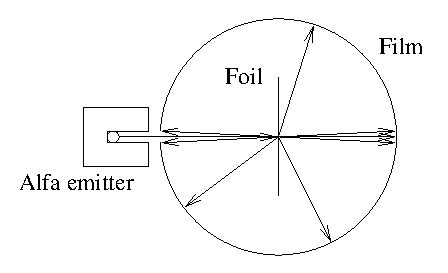
\includegraphics{rutherford}%
\end{picture}%
\setlength{\unitlength}{4144sp}%
%
\begingroup\makeatletter\ifx\SetFigFont\undefined%
\gdef\SetFigFont#1#2#3#4#5{%
  \reset@font\fontsize{#1}{#2pt}%
  \fontfamily{#3}\fontseries{#4}\fontshape{#5}%
  \selectfont}%
\fi\endgroup%
\begin{picture}(3159,1818)(-869,-970)
\end{picture}%
\caption{The Rutherford experiment.}\label{fig:rutherford}
\end{center}\end{figure}

However, over the years more particles were discovered: the positron (a positive electron), the neutrino, and the photon. Where did these fit into the model? With the development of (advanced) particle accelerators even more `elementary particles' were added to the list. The models became ever more complex and required a serious rethinking.

\section{Particles and Forces}
Objects, including particles like protons and electrons, exert forces upon each other. Some forces attract, others repel. We now know of four fundamental forces: The gravitational force (gravity for short), the electromagnetic force, the weak (nuclear) force and strong (nuclear) force. An object need not be in contact with another object to exert these forces, forces can work over long distances. They do so by exchanging particles, force carriers.

\begin{figure}\begin{center}
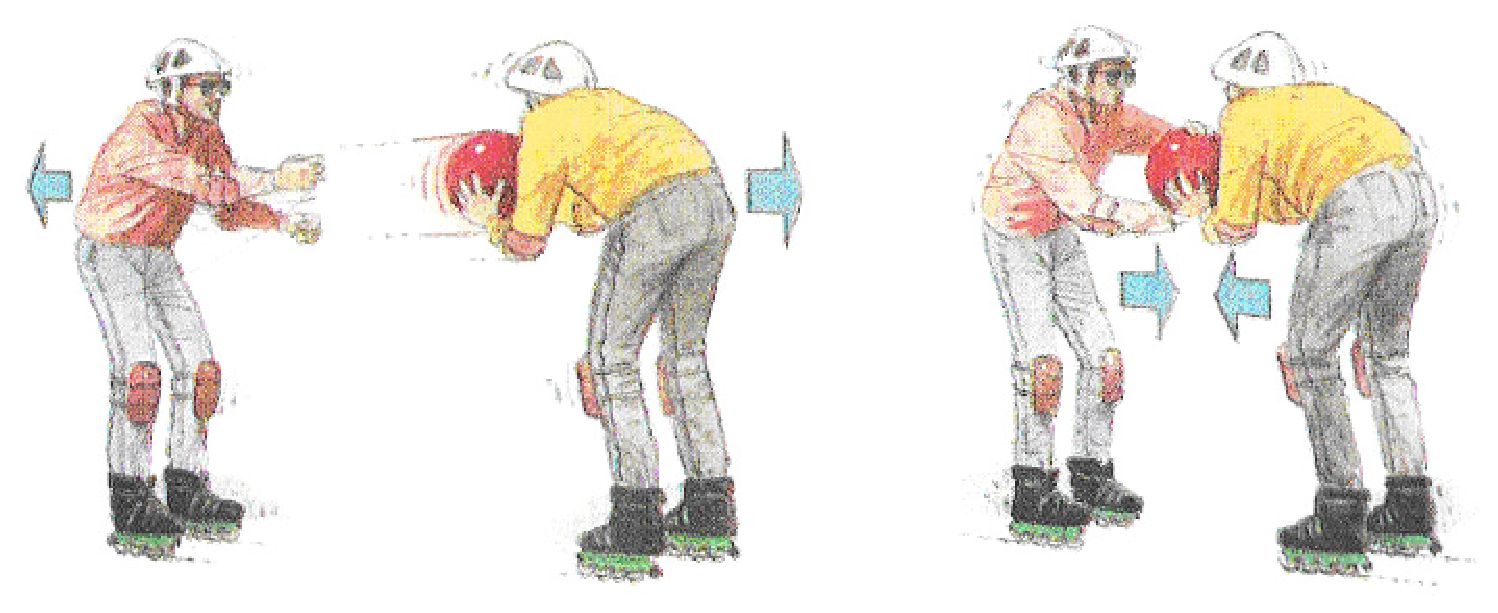
\includegraphics[scale=0.5]{force_particles.eps}%
\caption{Forces working between two bodies can compared to two skaters playing with a (heavy) ball. When one skater throws the ball to the other player who catches it, both will move away from each other. When both skates are pulling on the ball they move towards each other. Is this analogy the ball is the carrier of the force.}\label{fig:force_particles}
\end{center}\end{figure}

Hideki Yukawa is one of the first to put this idea of force carriers to paper. In 1935 he predicted the existence of a particle which must be responsible for the strong nuclear force; the force keeping protons and neutrons together inside the nucleus of an atom. He predicted that the mass of this particle should lie somewhere between the mass of the electron and proton. The aptly chosen name for this particle: meson (intermediate, in between).

Experiments with cosmic radiation revealed a particle with roughly the predicted mass; the mu meson. However, it turned out that this particle did not interact with other matter (as predicted) and could therefore not be the particle postulated by Yukawa. It lost its meson name and is now called the muon. In 1947 a different particle was discovered which did seem to fit the bill: the pi meson. This particle showed to have three different possible charges: $+e$, $-e$, and $0$. Pions are therefore abbreviated as: $\pi^+$, $\pi^-$, $\pi^0$. However, in 1970 it was revealed that mesons were not the carriers of the strong force (thus the pions also lost meson name), but a different particle was responsible: the gluon.

For every force there is an associated force particle. In the table below gives a summary of the fundamental forces and their carriers.

\begin{center}\begin{tabular}[h] {l l r l}
Force & Description & Relative & Force  \\
& & Strength & Carrier\\\hline
Strong force & force between protons  & 100 & gluon \\
& and neutrons inside nucleus\\
Electromagnetic force & force between charges & 1 & photon \\
& (electricity and magnetism) \\
Weak force & involved in radioactive decay & $10^{-11}$ & W$^\pm$, Z$^0$ \\
Gravitational force & force between masses & $10^{-36}$ & graviton \\
& & & (undiscovered)
\end{tabular}\end{center}
\captionof{table}{Fundamental forces and their carriers.}\label{tab:data_1}

\begin{shaded}
\textbf{Exercise \theExercise \stepcounter{Exercise}} : Table~\ref{tab:data_1} shows that gravity is by far the weakest force.
\begin{enumerate}[-]
\item Compare the gravitational force between two protons with the electrical force between the same particles. Do the same for a proton and an electron. Assume the two particles are suspended in an otherwise empty vacuum.
\item Explain why gravity can be felt at great distances.
\end{enumerate}\end{shaded}

\section{Particles and Anti-particles}
In 1932 a particle almost identical to the electron, except for the electrical charge, was discovered; the positron. It is the anti-particle of the electron. A single photon with enough energy can create an electron-positron pair. This process is called `creation' or `pair production'. During pair production the Energy $E$ of the photon is transformed into the combined mass $m$ of the two particles according to Einstein's famous equation:
\begin{equation}
E=m \cdot c^2
\end{equation}

The positron was only the first of many anti-particles to be discovered/created. When an anti-particle encounters its `regular' counterpart both are destroyed and their combined mass is transformed into energy. This process is called annihilation. During annihilation a pair of photons is created whose energy is determined by the same equation.

\section{Types of Particles}
A large number of different  particles have been discovered or created over the years. They can be classified according to their properties. The tree large groups are: bosons, leptons, and hadrons. The last group can be subdivided into two smaller groups: mesons and baryons. The table below gives a brief summary of the named groups.

\begin{center}\begin{tabular}[h] {l l}
Class & Particles \\ \hline
Bosons & Photon, W- and Z-particles \\
Leptons & electron, $e$-neutrino, muon, $\mu$-neutrino, tauon, and $\tau$-neutrino \\
hadrons: mesons & i.a.  pion \\
hadrons: baryons & i.a. proton and neutron
\end{tabular}\end{center}
\captionof{table}{Particle classes.}\label{tab:data_2}

\vspace{0.5cm}

Leptons are classified as elementary particles, i.e. they cannot be divided into smaller component particles. Their dimensions are so small they cannot be measured (\textless10$^{-18}$~m). We can therefore assume them to be point particles.

Hadrons were also thought to be elementary particles. But with more than a hundred different hadrons discovered, the list with elementary particles became very complex. Two men, Murray Gell-Mann and George Zweig, started to think about how baryons could be composed of smaller particles. In 1962 they proposed their theory of quarks. Quarks are named after (of at least their spelling is taken from) a line in the novel Finnegan's Wake by James Joyce: ``Three quarks for Muster Mark!''

Like the leptons, quarks are (as far as we now know) elementary particles. Like electrons, quarks are no larger than $10^{-18}$~m and can be seen as point particles. Both types of hadrons consist of quarks, the difference is that mesons contain two quarks whereas baryons contain three.

\section{Quarks}
We know of the existence of six different quarks (and another six anti-quark counterparts). They form pairs: up and down, charm and strange, and top and bottom. The table below gives a short summary. One thing you should immediately notice is the fractional charges of the quarks. In nature we only find integer charges (integer multiples of the electron or elementary charge).

\begin{center}\begin{tabular}[h] {l c r}
Name & Symbol & Charge ($e$) \\ \hline
up & u & $+\nicefrac{2}{3}$ \\
down & d & $-\nicefrac{1}{3}$ \\
charm & c & $+\nicefrac{2}{3}$ \\
strange & s & $-\nicefrac{1}{3}$ \\
top & t & $+\nicefrac{2}{3}$ \\
bottom & b & $-\nicefrac{1}{3}$ \\
\end{tabular}\end{center}
\captionof{table}{The six known quarks with their symbol and fractional charge.}\label{tab:data_3}

\vspace{0.5cm}

Both quarks and leptons are subdivided into three groups or generations. As shown in figure~\ref{fig:particles}. The first generation contains the up and down quarks as well as the electron and the electron-neutrino. Both the up and down quark are stable, they do not decay into other particles. Particles in the second and third generation have more mass than their first generation brothers. They are unstable and decay into lighter particles until they become particles from the first generation. We do not yet know if there are more than three generations of particles.

\begin{figure}[h]\begin{center}
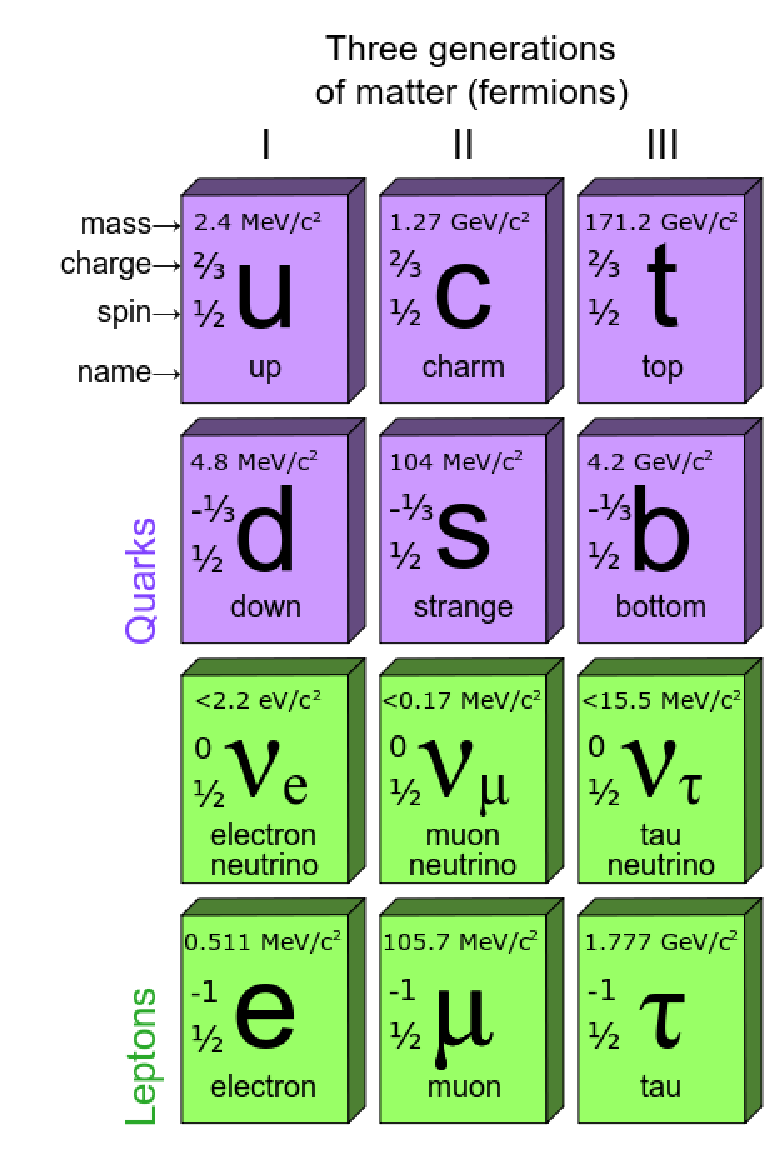
\includegraphics[scale=0.62]{particles.eps}%
\caption{The three generations of elementary particles.\protect\footnotemark}\label{fig:particles}
\end{center}\end{figure}
\footnotetext{Modified from \\ \url{http://en.wikipedia.org/wiki/File:Standard_Model_of_Elementary_Particles.svg}}

The anti-quarks are not included in table~\ref{tab:data_3} or figure~\ref{fig:particles}. As said earlier all properties of the anti-particle are the same for the regular particle except the charge, this property is the exact opposite. For instance, the anti-up-quark ($\overline{\mbox{u}}$) has a charge $-\nicefrac{2}{3}~e$.

Baryons consist of three quarks. To make a proton one needs two up- and one down-quark. A neutron has two down-quarks and one up-quark, or more concise: udd. Heavier (and therefore less stable) baryons consist of combinations with strange-, charm-, bottom-, or even top-quarks.

Mesons consist of only two quarks: one quarks and one anti-quark. The positive pion ($\pi^+$) is a combination of an up-quark with an anti-down-quark (u$\overline{\mbox{d}}$). The anti-particle of this meson, $\pi^-$, has the reverse combination of quark and anti-quark: $\overline{\mbox{u}}$d. The neutral pion, $\pi^0$ is a combination or mix of u$\overline{\mbox{u}}$ and d$\overline{\mbox{d}}$. Because mesons are combinations of matter with anti-matter they highly unstable. 

\begin{shaded}
\textbf{Exercise \theExercise \stepcounter{Exercise}} : Use the charges of quarks listed in table~\ref{tab:data_3} to verify the charges of the proton, neutron, and the three pions.\end{shaded}

One of the holy grails in physics is the unification of all fundamental forces. This process started with the insight that magnetism and electricity are one and the same force. Physicists have so far been successful in combining the electromagnetic force and the weak force into one model: the Standard Model. This model contains the six quarks, six leptons, and the force carriers.

\section{Proton-Proton Collisions}
What happens when a high energetic cosmic particle collides with the nucleus of an oxygen or nitrogen atom high up in the atmosphere? Lets assume the cosmic ray is a proton and that it hits one of the other protons inside the nucleus. When the incident proton has enough energy then (a part of) this energy can be converted into mass. In a similar fashion to the pair creation of an electron and a positron by a photon, the proton can create a quark anti-quark pair. There are two possible outcomes:
\begin{itemize}
\item The creation of a neutral pion ($\pi^ 0$): $\isotope[1][1]{p} + \isotope[1][1]{p} \rightarrow \isotope[1][1]{p} + \isotope[1][1]{p} + \pi^0$
\item The creation of a charged pion and a neutron: $\isotope[1][1]{p} + \isotope[1][1]{p} \rightarrow \isotope[1][0]{n} + \isotope[1][1]{p} + \pi^+$
\end{itemize}

\begin{shaded}
\textbf{Exercise \theExercise \stepcounter{Exercise}} : Which quarks are created in the two processes described above? Do the existing quarks stay in their place or are they rearranged? \end{shaded}

The neutral $\pi^0$ pion has a very short life-time of only $0.84 \cdot 10^{-16}$~s after which it decays into photons. The mass of the pion is thus converted directly into energy. The positive $\pi^+$ pion is a little more stable. It has a life-time of $2.60 \cdot 10^{-8}$~s and decays into a (unstable) muon and a (stable) neutrino. The muon in turn decays into a stable electron and two neutrinos.

\section{Quark-Gluon Plasma}
High energetic particles coming from all over the cosmos which are hitting the outer layer of the atmosphere can create such violent events that a new type of phase transition occurs: the creation of a quark-gluon plasma. As we saw in the previous sections quarks are the building blocks of the protons and neutrons. They are held together by gluons (`glue particles'). But the gluons also bind the protons and neutrons together inside the nucleus, the strong nuclear force is strong enough to hold the repelling charges of the protons together.

Figure~\ref{fig:quark_gluon} shows the phase transition from normal matter to a quark-gluon plasma and back to normal matter. In normal matter quarks are bound in sets of three (or two when we look at mesons), but under extremely high pressure and equally extreme temperatures a new state arises in which the quarks and gluons are free to move: the quark-gluon plasma.

\begin{figure}\begin{center}
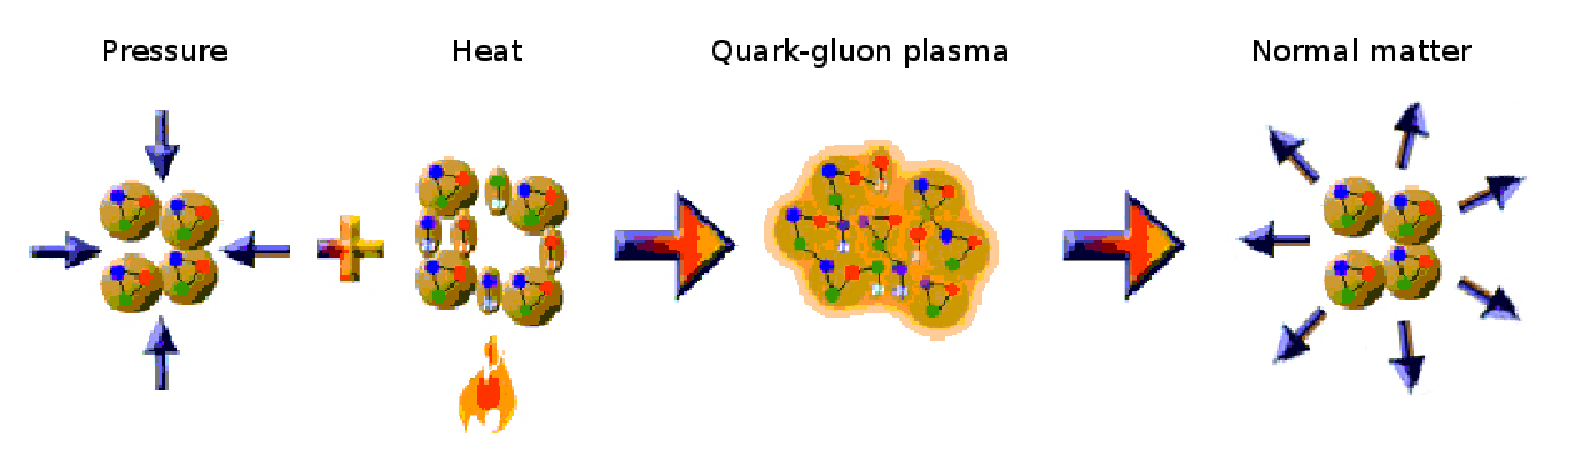
\includegraphics[scale=0.6]{quark_gluon.eps}%
\caption{Schematic representation of the formation of a quark-gluon plasma, followed by the return to normal matter.}\label{fig:quark_gluon}
\end{center}\end{figure}

Cosmic radiation consist mainly of protons. In the upper layers of the atmosphere nitrogen atoms are the most prevalent. High energetic collisions between the two will most likely not create a quark-gluon plasma. This is because the cosmic proton only interacts with one of the nucleons (proton or neutron) inside the nitrogen atom. To create the quark-gluon plasma large numbers of protons and/or neutrons must be involved. Only under very specific conditions can cosmic radiation involve larger numbers of nucleons in a single interaction.

One such instance is when a heavier cosmic nucleus, such as an iron core, interacts with a nitrogen atom. Unfortunately this type of cosmic radiation is very rare; at most one particle per square metre per year. Moreover, the type of interaction must be of a specific type: frontal and inelastic.\footnote{See the module `Collisions' for more information about the different types of interactions.} Only during such a collision enough protons and/or neutrons are involved in the interaction to create the necessary energy density of 1.5~GeV/fm$^3$. The minimal (critical) temperature to create a quark-gluon plasma is 120~MeV,\footnote{In plasma physics and a number of other fields it is customary to express temperature in electronvolts, 1~eV~=~11,605~K.} over 10$^{11}$~K. The pressure inside the plasma is $\approx 3 \cdot 10^33$~N/cm$^2$, the weight of thirty suns on one square centimetre!

Because the extreme (local) heat and pressure the plasma expands with $\approx 0.5 \cdot c$. Temperature and pressure rapidly decrease until the plasma returns to normal matter containing neutrons and protons.

Why the interest for this special state of matter? The current working theory is that our universe started with the Big Bang. After the `birth' of the universe there was a very short time when there was only this quark-gluon plasma before normal matter was formed. By studying this plasma we might learn more about how the universe was formed. A second area of interest comes from the study of neutron  stars (and the as of yet hypothetical quark stars). Physicists and astronomers suspect that the core of these types of stars consists of quark-gluon plasma.
 
\end{document}
